\section{Method: AgentSpec}
\begin{figure}[ht]
\centering
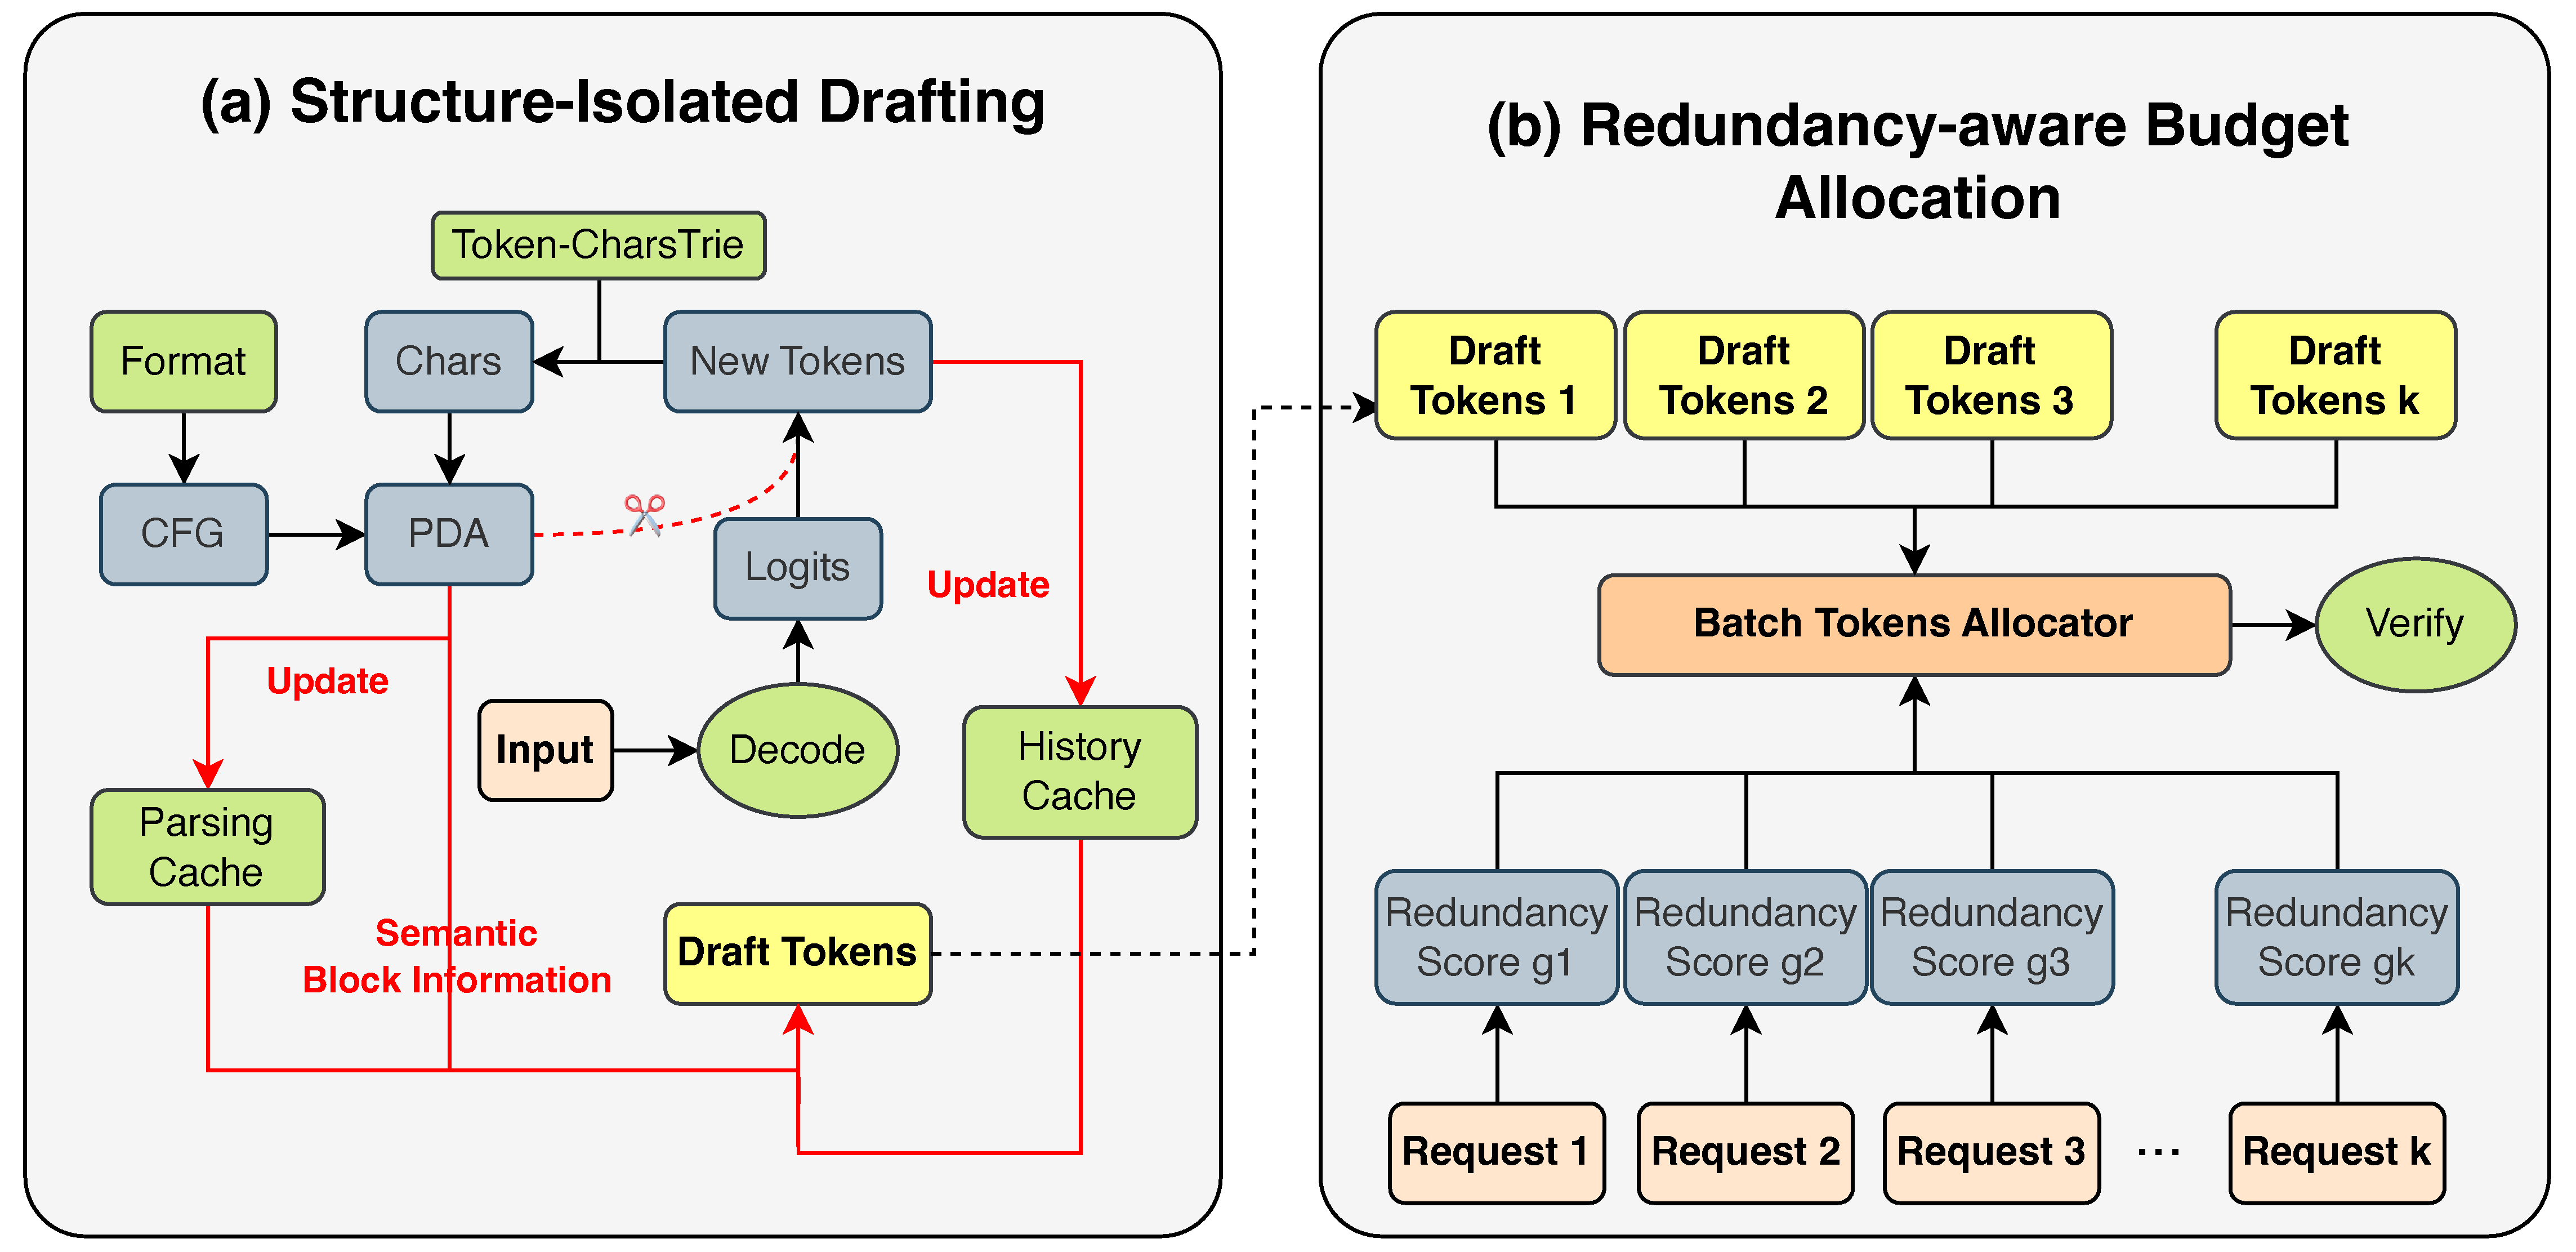
\includegraphics[width=0.48\textwidth]{Figures/AgentSpec.pdf}
\caption{Overview of \sysname.}
\label{fig:overview}
\end{figure}
\label{sec:method}
% \xin{Figure provides an overview of \sysname. }
The overview of \sysname is provided in~\cref{fig:overview}. At a high level, \sysname is a model-free speculative decoding algorithm designed for LLM agents. It requires the agent application to provide an agentic structure identifier alongside the input prompt to the LLM server, which enables the system to organize and retrieve historical context according to agent-specific execution structure.
%
During speculative drafting, \sysname retrieves draft candidates only from historical segments that belong to the same semantic group, thereby avoiding speculation across structurally mismatched contexts. Before verification, \sysname computes an integrated redundancy value for each request in the batch by combining local draft information with global generation history. It then allocates speculative token budgets across requests according to their relative redundancy scores and adjusts the draft length of each request accordingly.
%
In the following, we describe the two key components of \sysname—structure-isolated drafting and redundancy-aware budget allocation—in detail.


\subsection{Structure-Isolated Drafting}

\label{subsec:structured_isolated_drafting}
\noindent\textbf{Motivation:}
% 相同session的history matching数量 >> 不同session的history matching数量
% 相同session的相同sementic block内history matching的数量 >> 相同session的不同sementic block内history matching的数量
A key distinction between LLM agent applications and standard LLM workloads is that a single user query often spans multiple requests associated with different semantic blocks (e.g., reasoning, tool execution, and result interpretation). While generation patterns are highly consistent within the same semantic block, transitions across blocks or queries introduce substantial semantic shifts.

To quantify this effect, we analyze generation trajectories of Qwen-3-8B on the USACO dataset using a Reflexion-based code generation agent. For each request, we measure repeated token segments that reappear in previously generated content, distinguishing repetitions within the same block from those across different blocks or queries. A repetition is counted only if it contains at least $k$ consecutive tokens, with overlapping matches merged into their longest contiguous span. As shown in~\cref{fig:moti_repeated_ratio}, repeated token segments overwhelmingly occur within the same semantic block of a single query, whereas cross-block and cross-query repetitions are rare. This observation indicates that speculative drafting can be substantially improved by being aware of semantic block boundaries and query scope, thereby reducing unnecessary drafting and speculative rejections. In contrast, existing methods such as NGram and SuffixDecoding retrieve draft candidates from global generation history without such distinctions, leading to high rejection rates and wasted verification cost in agentic workloads.
\begin{figure}[t]
\centering
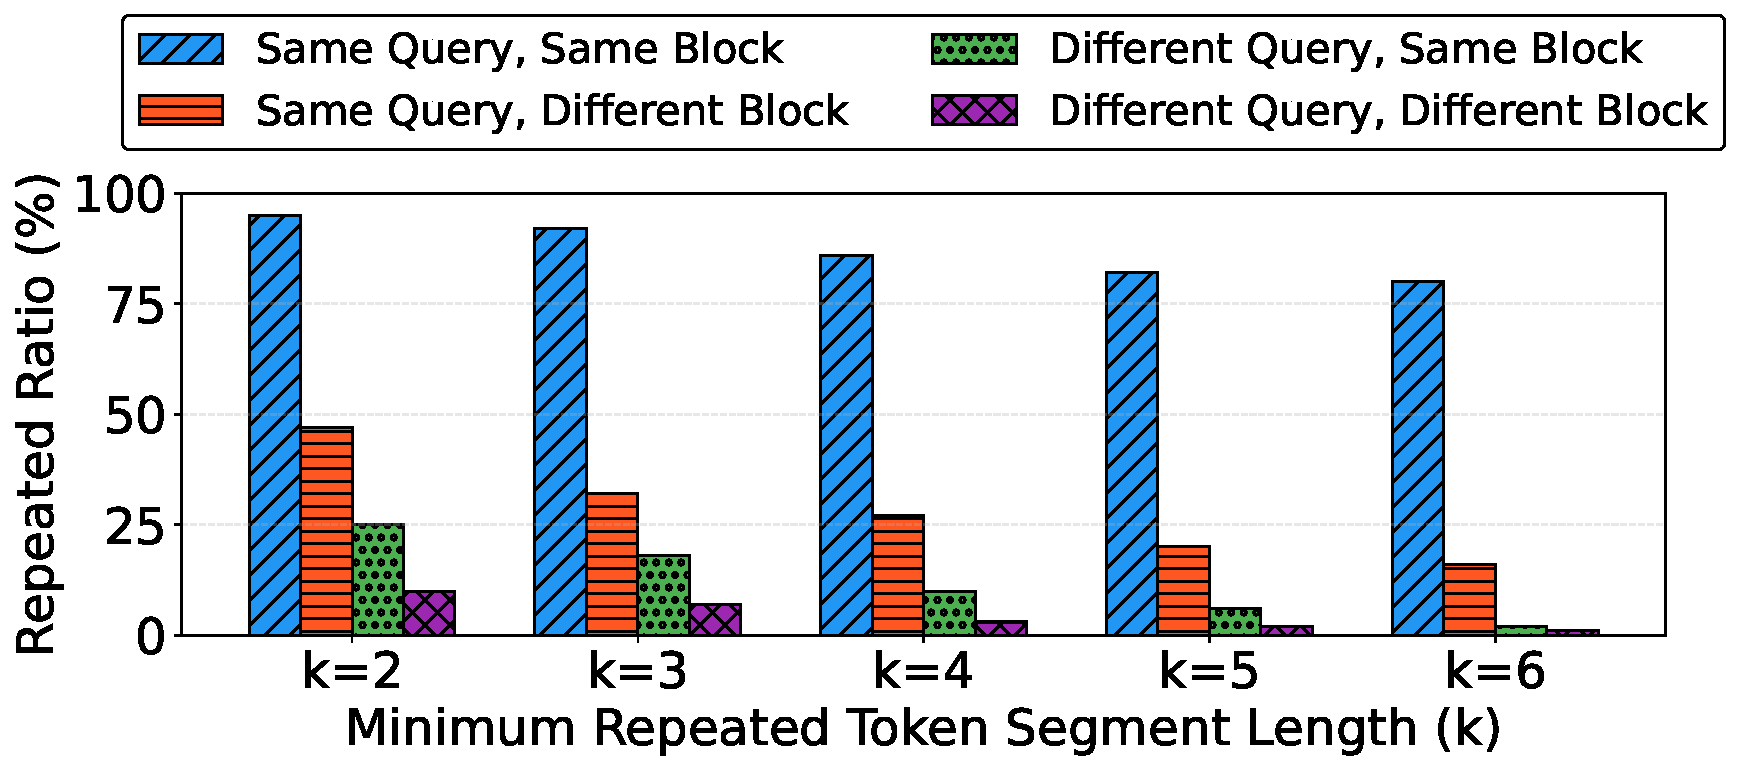
\includegraphics[width=0.48\textwidth]{Figures/moti_repeated_ratio.pdf}
\caption{Repeated token ratio under different minimum repeated span lengths $k$. The repeated ratio is defined as the total length of maximal repeated segments with at least $k$ consecutive tokens appearing in historical generations, normalized by the total generation length. Repetitions are categorized by whether they occur under the same or different user queries and within the same or different semantic blocks.}

\label{fig:moti_repeated_ratio}
\end{figure}

\noindent\textbf{Key Design:}
The pseudocode of structured-isolated draft of \sysname is provided in~\cref{algo:structure_isolated_drafting}. As shown, the algorithm requires the agent application to explicitly provide semantic structure identifier $S_i$ together with each generation request $r_i$ as below:
$$S_i=\{a_i, q_i, B_i\}$$
where $a_i$ denotes the agent application identifier, $q_i$ denotes the user query index that triggers the current request, and $b_i$ represents the list of $n$ semantic blocks $B_i = [b_i^1, b_i^2, b_i^3,...,b_i^n]$, defined by pairs of start and end string tags identified from previous generation history.

Mapping string-level semantic blocks to token-level generation is challenging due to subword tokenization, where token boundaries do not align with string boundaries. Direct token–string conversion during decoding is prohibitively expensive in common serving engines such as vLLM and sglang, where tokenization and decoding are handled by separate components.

To address this, \sysname adopts a design similar to XGrammar~\citep{DBLP:conf/mlsys/DongRCXZL025} by maintaining a cached token-to-string mapping $M$, enabling efficient online conversion of generated tokens without invoking the tokenizer. Based on this mapping, \sysname maintains a lightweight string-based pushdown automaton (PDA) $P$ on the server, which is incrementally updated to track the current semantic block.

For each request $r_i$, newly generated tokens are converted using $M$ and fed into the corresponding PDA $P(a_i, q_i)$ to identify the active semantic block $b_i^k$. \sysname maintains a separate structure-isolated cache for each semantic block and retrieves speculative drafts exclusively from the matched block, avoiding semantically irrelevant contexts and substantially reducing speculative rejections. As shown in~\cref{tab:rejection_rate}, \sysname achieves a rejection rate as low as 26\%, over 2$\times$ lower than existing baselines.


\subsection{Redundancy-aware Budget Allocation}
\label{subsec:redundancy_aware_budget_allocation}
\noindent\textbf{Motivation:} The pseudocode of the redundancy-aware budget allocation is shown in~\cref{algo:redundancy_aware_budget}.
To efficiently utilize the dynamic token budget in speculative decoding, more draft tokens should be assigned to requests with higher acceptance potential. Over-allocating tokens to low-acceptance requests wastes verification cost, while overly conservative allocation under-utilizes the available budget. The key challenge is thus to identify a reliable request-level signal that predicts draft acceptance.
%
In agent workloads, requests exhibit varying degrees of redundancy in their generation history. Intuitively, drafts aligned with repeated historical patterns are more likely to be accepted. To validate this intuition, we analyze generation traces from Qwen-3-8B on Code Generation Agent and measure draft redundancy as the fraction of matched historical continuations that fully accept the draft. As shown in~\cref{fig:redundancy_accept_map}, higher redundancy strongly correlates with higher acceptance rates, with the correlation strengthening as more matched continuations are observed.

\begin{figure}[t]
\centering
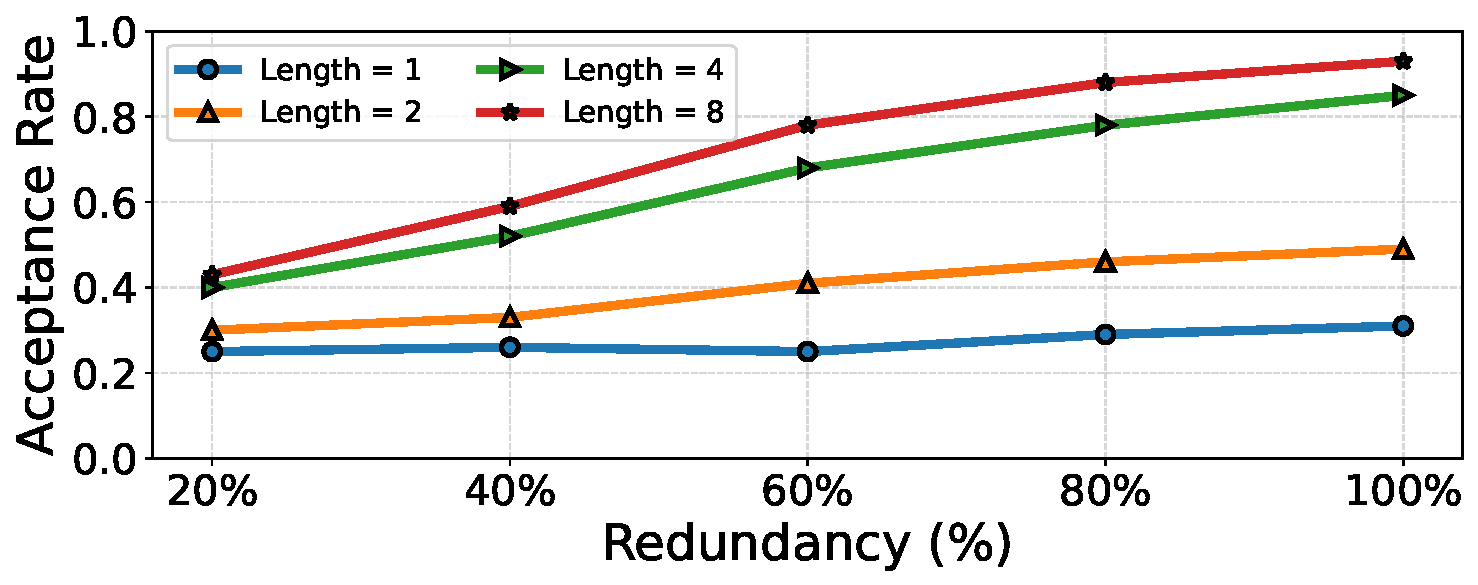
\includegraphics[width=0.48\textwidth]{Figures/redundancy_accept.pdf}
\caption{Acceptance ratio ($1-\rho(b)$ under different redundancy ratio with different matching pattern length.}
\label{fig:redundancy_accept_map}
\end{figure}

% 相同agent应用的接受率相近， 不同的差异明显
% 越一致，接受率越高 more consensus, more probable to accept
% model free的方法都是用continuation来做的

\noindent\textbf{Key Design:} 
% To estimate the acceptance likelihood of a speculative draft for each request in a batch, \sysname introduces a redundancy score $g$, defined as:
% \begin{equation}
% g(c, n)=\frac{c}{n} \cdot p(n)=\frac{c}{n} \cdot\left[g_{\min }+\left(1-g_{\min }\right)\left(1-e^{1-n}\right)\right]
% \end{equation}
% where $n$ denotes the number of candidate continuations found in the generation history under the same semantic block and the same user query, and $c$ denotes the number of continuations that agree on the most frequent continuation prefix. The hyperparameter $g_{min}$ controls the minimum confidence when historical evidence is scarce.
%
% The ratio $\frac{c}{n}$ captures the consensus among candidate continuations: a larger value indicates higher redundancy and a higher likelihood that the proposed draft will be accepted. However, empirical results in the motivation part show that when $n$ is small, acceptance rates remain low even if $\frac{c}{n}$ is large. To account for this effect, we introduce the exponential saturation term $p(n)$, which downweights redundancy estimates under low-support scenarios.
%
% Given the redundancy scores, \sysname computes the total speculative token budget as
% \begin{equation}
% B_t=\left\lfloor\frac{\alpha}{b z}\right\rfloor
% \end{equation}
% where $bz$ is the current batch size and $\alpha$ is a tunable hyperparameter that controls the overall speculative budget. For each request $r_i$ in the batch, \sysname retrieves all $n_i$ candidate draft paths from the history that belong to the same semantic block and user query. A lightweight n-gram index is then constructed to identify the most frequent continuation prefix $CT_i$ and compute its redundancy score $g_i$. After obtaining ${(CT_i, g_i)}$ for all requests, \sysname allocates a per-request draft length
% \begin{equation}
% L_i=\max \left(\left|C T_i\right|, B_t \cdot \frac{g_i}{\sum_j g_j}\right)
% \end{equation}
% prioritizing requests with higher redundancy while ensuring that each request can draft at least its most confident continuation prefix. As shown in~\cref{fig:moti_token_number}, \sysname consistently ensures a batch draft token number lower than the maximum budget $M(b)$, and generally approaches it with the increase of batch size, indicating a good utilization of the available token budget during agent batch inference.
To estimate the acceptance likelihood of a speculative draft for each request,
\sysname introduces a redundancy score $g$:
\begin{equation}
g(c,n) = \frac{c}{n}\cdot p(n), \;
p(n) = g_{\min} + (1-g_{\min})(1-e^{1-n}),
\end{equation}
where $n$ is the number of candidate continuations retrieved from the generation
history under the same semantic block and user query, and $c$ is the number of
continuations agreeing on the most frequent prefix. The ratio $c/n$ captures the
consensus among candidates, while the saturation term $p(n)$ downweights unreliable
estimates when historical support is limited. The hyperparameter $g_{\min}$ controls
the minimum confidence under low-support scenarios.

Given the redundancy scores, \sysname computes the batch-level speculative token
budget as
\begin{equation}
B_t = \left\lfloor \frac{\alpha}{bz} \right\rfloor,
\end{equation}
where $bz$ is the batch size and $\alpha$ controls the overall speculative budget.
For each request $r_i$, \sysname retrieves candidate drafts within the same semantic
block and query, identifies the most frequent continuation prefix $CT_i$, and
computes its redundancy score $g_i$. The per-request draft length is then allocated as
\begin{equation}
L_i = \max\!\left(|CT_i|,\; B_t \cdot \frac{g_i}{\sum_j g_j}\right),
\end{equation}
prioritizing requests with higher redundancy while ensuring that each request can
draft at least its most confident prefix.

As shown in~\cref{fig:moti_token_number}, \sysname consistently keeps the total number
of drafted tokens below the maximum budget $M(b)$ and approaches it as batch size
increases, indicating effective utilization of the available speculative budget.
